\documentclass{amsart}

\usepackage{tikz}
\usepackage{amsmath}
\usetikzlibrary{fit,arrows,calc,positioning,shapes,arrows,arrows.meta}

\definecolor{heavyorange}{HTML}{FF7600}
\definecolor{almostblack}{HTML}{1a0f00}
\definecolor{lightorange}{HTML}{ffebcc}
\definecolor{lightgrey}{HTML}{f6f6f6}
\begin{document}
 
\begin{center}	
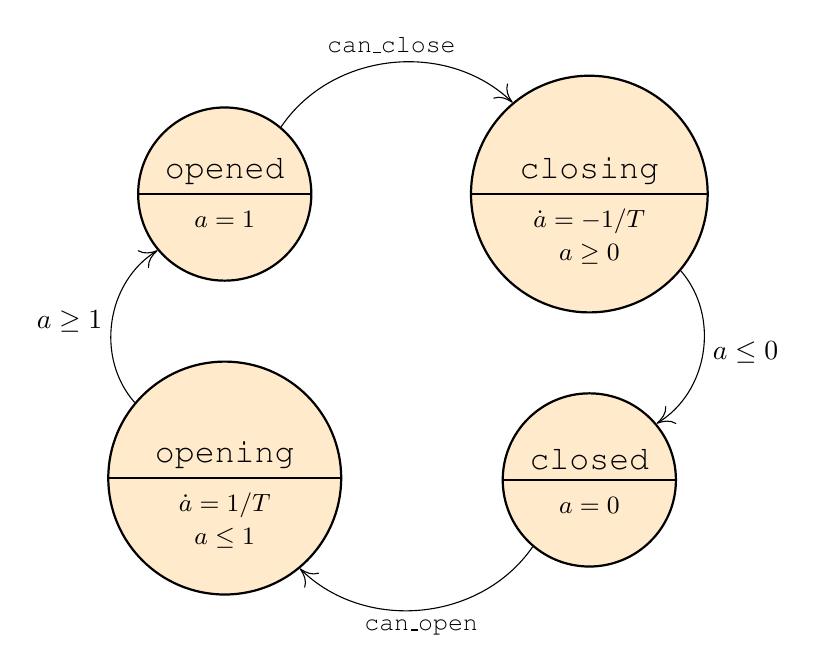
\begin{tikzpicture}
   \node[circle split, draw, thick, fill=lightorange] (opened)
   {\fontfamily{pcr}\selectfont \large opened \nodepart{lower} 
   \begin{tabular}{c}
   \small $a = 1$
   \end{tabular} 
   };
   \node[circle split, draw, thick, fill=lightorange] (closing) [right=2 cm of opened] 
   {\fontfamily{pcr}\selectfont \large closing \nodepart{lower} 
   \begin{tabular}{c}
   \small $\dot{a} = -1/T$ \\ 
   \small $a \geq 0$
   \end{tabular} 
   };
   \node[circle split, draw, thick, fill=lightorange] (closed) [below=1 cm of closing] 
   {\fontfamily{pcr}\selectfont \large closed \nodepart{lower} 
   \begin{tabular}{c}
   \small $a = 0$
   \end{tabular} 
   };
   \node[circle split, draw, thick, fill=lightorange] (opening) [below=1 cm of opened] 
   {\fontfamily{pcr}\selectfont \large opening \nodepart{lower} 
   \begin{tabular}{c}
   \small $\dot{a} = 1/T$ \\ 
   \small $a \leq 1$
   \end{tabular} 
   };
    \path[-{>[scale=2.5, width=3]},line width=0.4pt]
     (opened) edge[bend left=50] 
       node[anchor=north,above]{\fontfamily{pcr}\selectfont \small can\_close} (closing)                  
     (closing) edge[bend left=50]  
       node[anchor=west]{$a \leq 0$} (closed)
     (closed) edge[bend left=50] 
       node[anchor=south,below]{\fontfamily{pcr}\selectfont \small can\_open} (opening)       
     (opening) edge[bend left=50]  
       node[anchor=east]{$a \geq 1$} (opened)            
     ;
\end{tikzpicture}
\end{center}

	
\end{document}